
\chapter{Implementation of Balancing Circuit}

\indent\indent The implementation of this project was done using a battery monitoring \acrshort{ic} from Texas Instruments in a custom designed printed circuit board and Li-ion cells. The hardware is divided into two parts,a master board which is the STM32F103C8T6 microcontroller and the module board which consists of the BQ76PL455A battery monitoring IC and the balancing circuit.  



\section{BQ76PL455A-Q1}
The BQ76PL455A-Q1 device is an integrated 16-cell battery monitoring and protection device from Texas Instruments, designed for high-reliability automotive applications. The integrated high-speed, differential, capacitor-isolated communications interface allows up to sixteen BQ76PL455A-Q1 devices to communicate with a host via a single high-speed Universal Asynchronous Receiver/Transmitter (\acrshort{uart}) interface \cite{ti:pl455}.

\begin{figure}[!h]
    \centering
    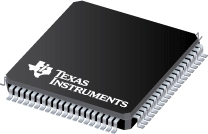
\includegraphics[]{Chapter4/BQ76PL455A-Q1.jpg}
    \caption{BQ76PL455A-Q1 \acrshort{ic} from Texas Instruments \cite{ti:pl455}}
   
\end{figure}
The features of this \acrshort{ic} are 

\begin{itemize}
    \item Monitors and Balances 6-to-16 Cells per Device
    \item High Performance 14-bit Analog-to-Digital Converter (\acrshort{adc}) With Internal Reference 
    \item All Cells Converted in 2.4 ms (Nominal)
    \item Passive Balancing with External n-FETs
    \item Up to 16 ICs in Daisy-Chain With Twisted Pair
\end{itemize}

\section{Hardware Design}

The hardware design was done using a open source PCB designing software called KiCAD. The design process consisted of following steps

\begin{itemize}
    \item Schematic generation
    \item Placement and Routing 
    \item Fabrication and Assembly
\end{itemize}

\subsection{Schematic generation}
The schematic was developed based on the results obtained in the MATLAB simulations.The snapshots of the schematic are shown below
\begin{figure}[!h]
    \centering
    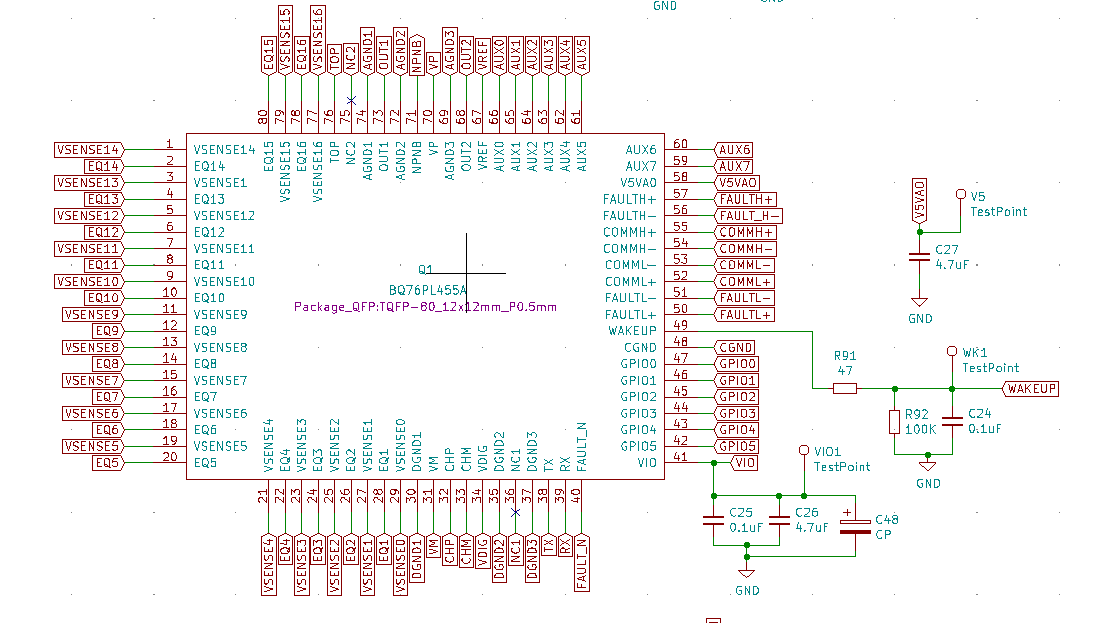
\includegraphics[scale=0.5]{Chapter4/Screenshot (53).png}
    \caption{Battery monitoring \acrshort{ic}}
\end{figure}

Figure 4.2 shows the snapshot of the schematic which shows how the monitoring \acrshort{ic} is integrated with other parts of the circuit.

\begin{figure}[H]
    \centering
    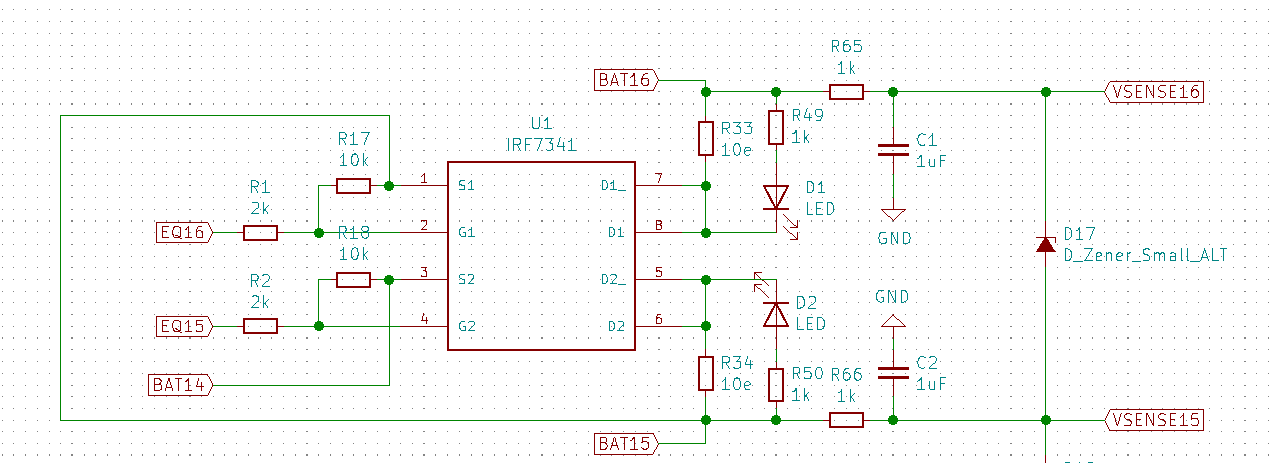
\includegraphics[scale=0.5]{Chapter4/Screenshot (55).png}
    \caption{Bleeding circuit}
\end{figure}

Figure 4.3 shows the bleeding circuit which is responsible for balancing the cells. It consists of IRF7341 which is a dual mosfet \acrshort{ic} from Infineon.

\subsection{Placement and Routing}

After successfully completing the schematic placement and routing of the components in the PCB is done. Figure 4.4 shows the fully routed PCB and Figure 4.5 shows the ECAD model rendered in KiCad.

\begin{figure}[H]
    \centering
    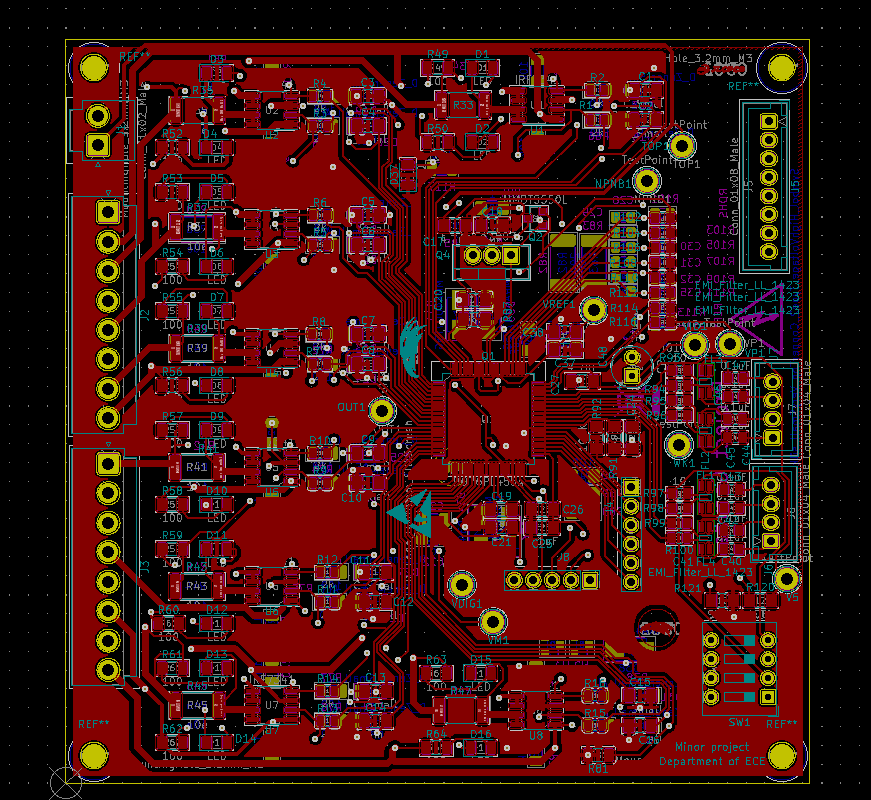
\includegraphics[scale=0.5]{Chapter4/Screenshot (56).png}
    \caption{Fully routed PCB}
\end{figure}

\begin{figure}[H]
    \centering
    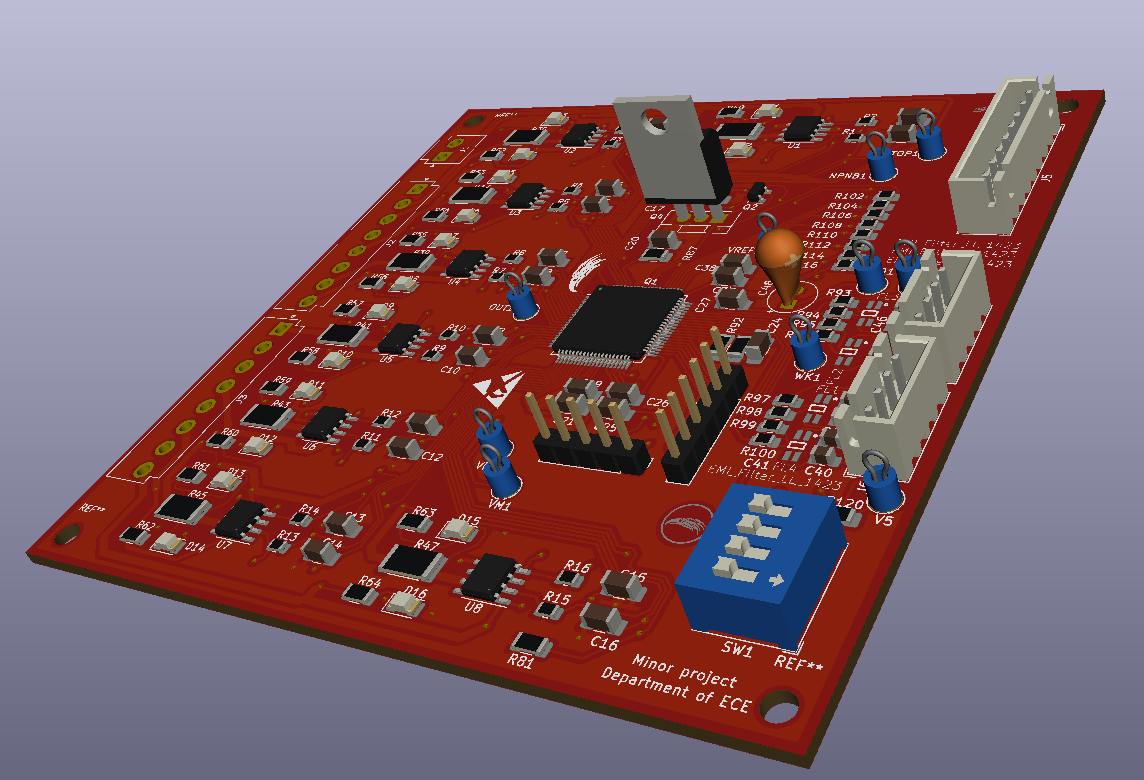
\includegraphics[scale=0.4]{Chapter4/Screenshot (57).png}
    \caption{ECAD Model of the PCB}
\end{figure}


\subsection{Fabrication and Assembly}

After successfully routing, the PCB was sent for fabrication following which the assembly of all the components was done.

Figure 4.6 shows the assembled PCB.
\begin{figure}[H]
    \centering
    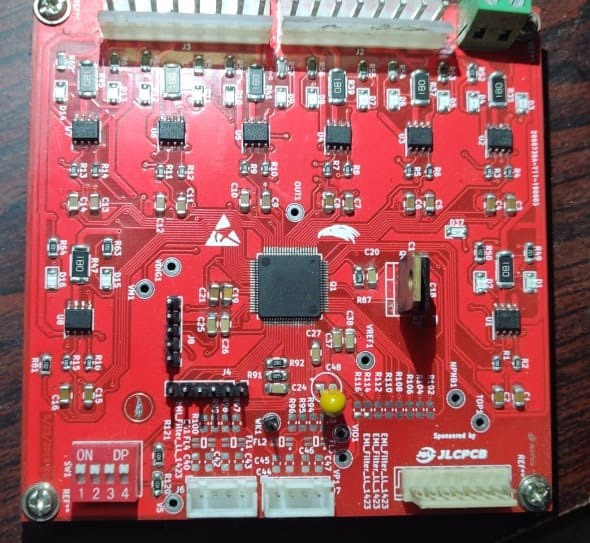
\includegraphics[scale=0.8]{Chapter4/assembly.jpg}
    \caption{Assembled PCB}
\end{figure}

\section{Testing}

The assembled PCB was tested for functionality  with the setup shown in figure 4.7.
\begin{figure}[H]
    \centering
    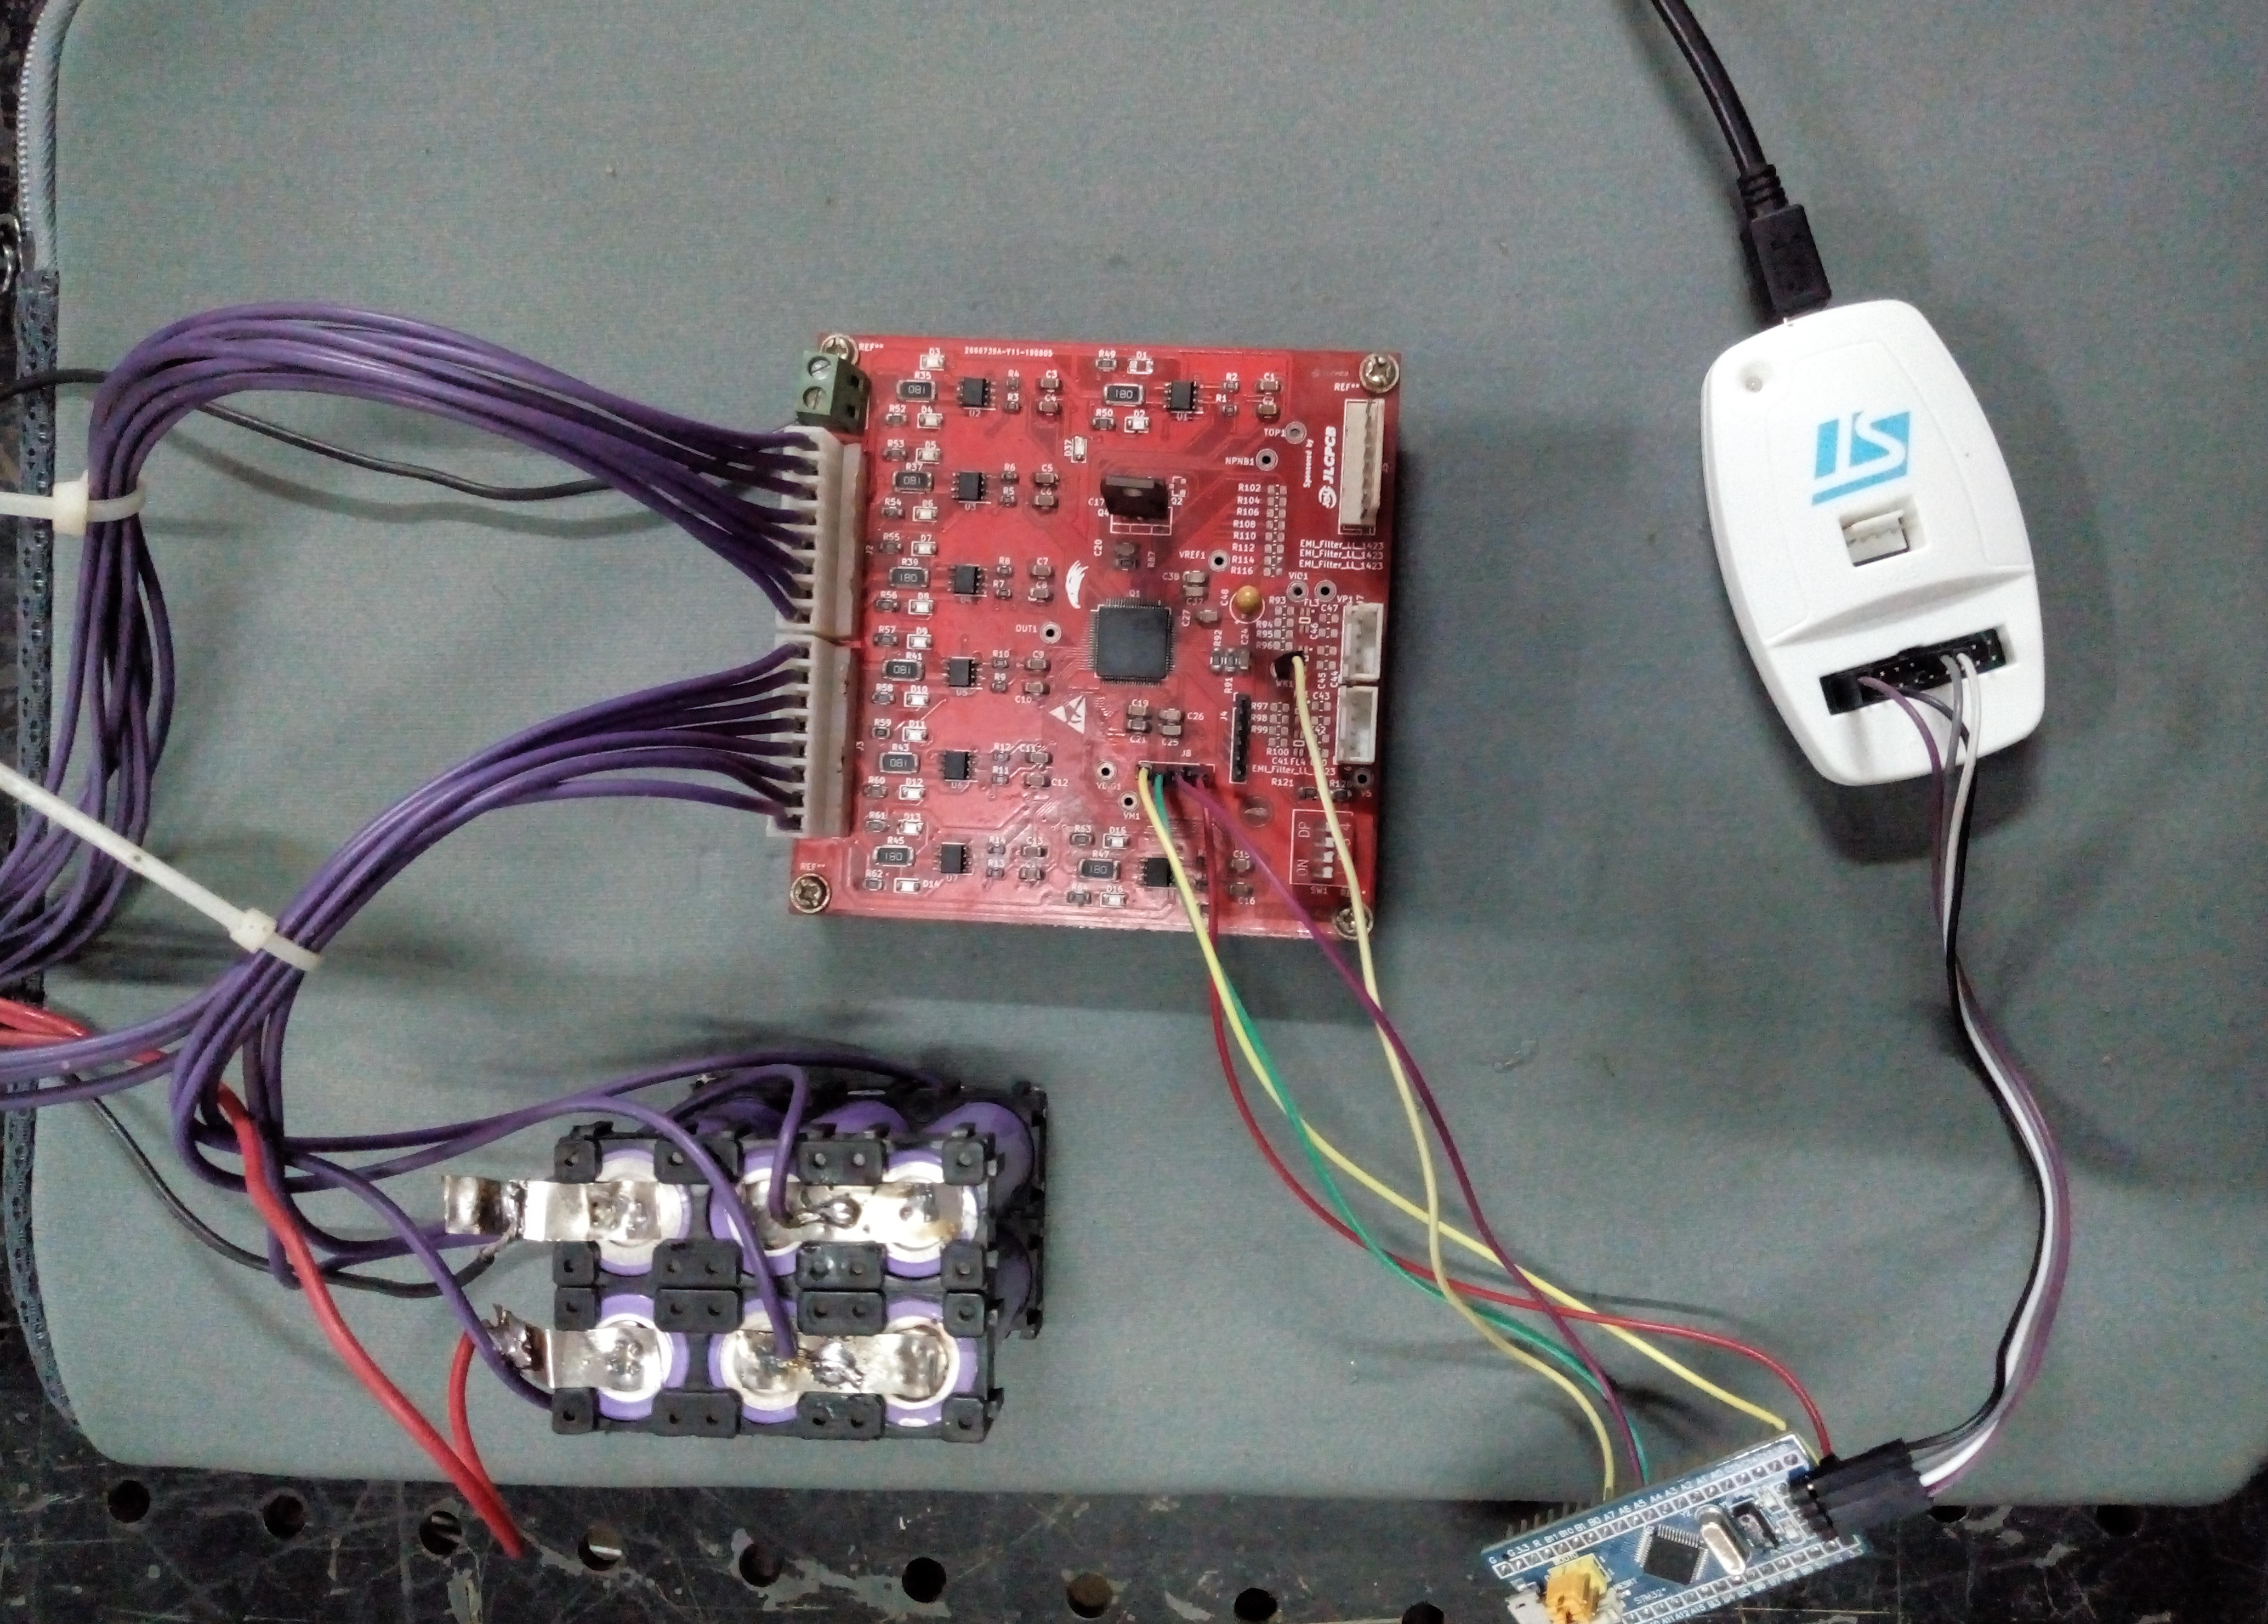
\includegraphics[scale=0.1]{Chapter4/IMG_20210110_205116558 (2).jpg}
    \caption{Testing setup}
\end{figure}

\section{Host micro-controller and Embedded Software }
\indent The host micro-controller used in this project is the STM32F103C8T6 from ST microelectronics\textsuperscript{\textregistered}. 

\subsection{STM32F103C8T6}
The STM32F103C8T6 is a medium density performance line chip housing ARM\textsuperscript{\textregistered} Cortex-M3 32bit microcontroller in 48 pin LQFP package. It incorporates high performance RISC core with 72MHz operating frequency and 1.25 DMIPS/MHz, high speed embedded memories, extensive range of enhanced I/Os and peripherals connected to two APB buses. The STM32F103C8T6 features 12bit \acrshort{adc}, timers, PWM timer, standard and advanced communication interfaces. A comprehensive set of power saving mode allows the design of low power applications \cite{stm:bluepill}.

\begin{figure}[!h]
    \centering
    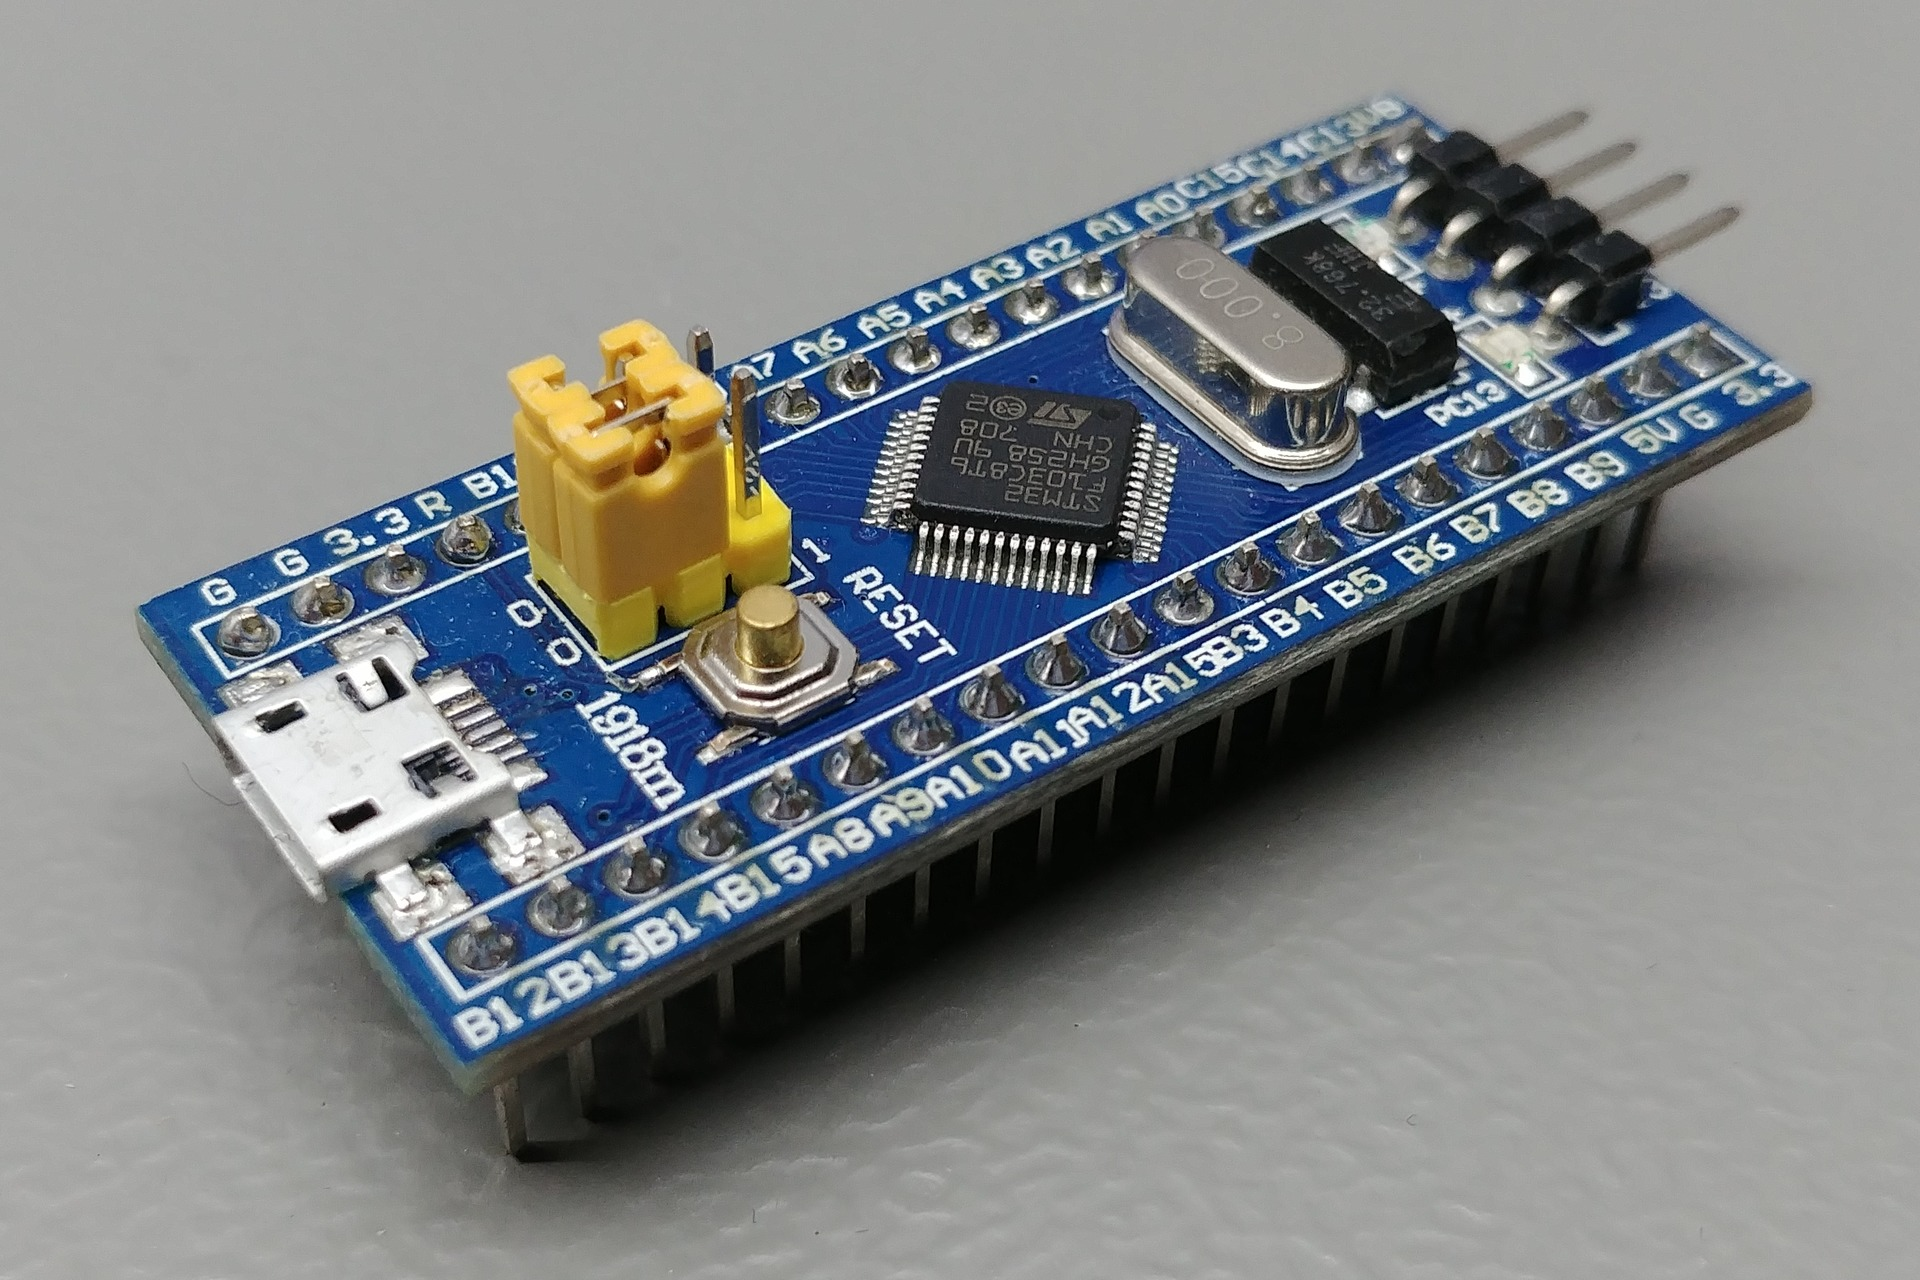
\includegraphics[scale=0.5]{Chapter4/STM32F103C8T6_Blue_Pill-1.jpg}
    \caption{STM32F103C8T6 - Blue Pill Development Board}
\end{figure}

It's development board named Blue pill is readily available in market for testing. And it has got required number of GPIOs and \acrshort{uart} peripherals required for the project.It comes with a micro USB port which can be used to power it and the board is  Arduino\textsuperscript{\textregistered} IDE compatible with bootloader loaded in one can code the chip using an external USB/Serial converter connected to UART1 pins. Otherwise STLink\textsuperscript{\textregistered} USB Dongle needs to be used for single-wire debug interface to communicate with the board. This allows it to be programmed using advanced software like Keil\textsuperscript{\textregistered}/CubeIDE\textsuperscript{\textregistered}. It allows memory access to internal registers/memory of the microcontroller hence enabling debugging features for developers.

\subsection{STM32CubeMX}

STM32CubeMX is a graphical tool developed by ST Microelectronics which allows easy configuration of STM32 microcontrollers and microprocessors. And it also gene
that allows a very easy configuration of STM32 microcontrollers and microprocessors, as well as the generation of the corresponding initialization C code for the Arm\textsuperscript{\textregistered} Cortex\textsuperscript{\textregistered}-M core or a partial Linux\textsuperscript{\textregistered} Device Tree for Arm\textsuperscript{\textregistered} Cortex\textsuperscript{\textregistered}-A core \cite{stm:cubemx}.

\begin{figure}[!h]
    \centering
    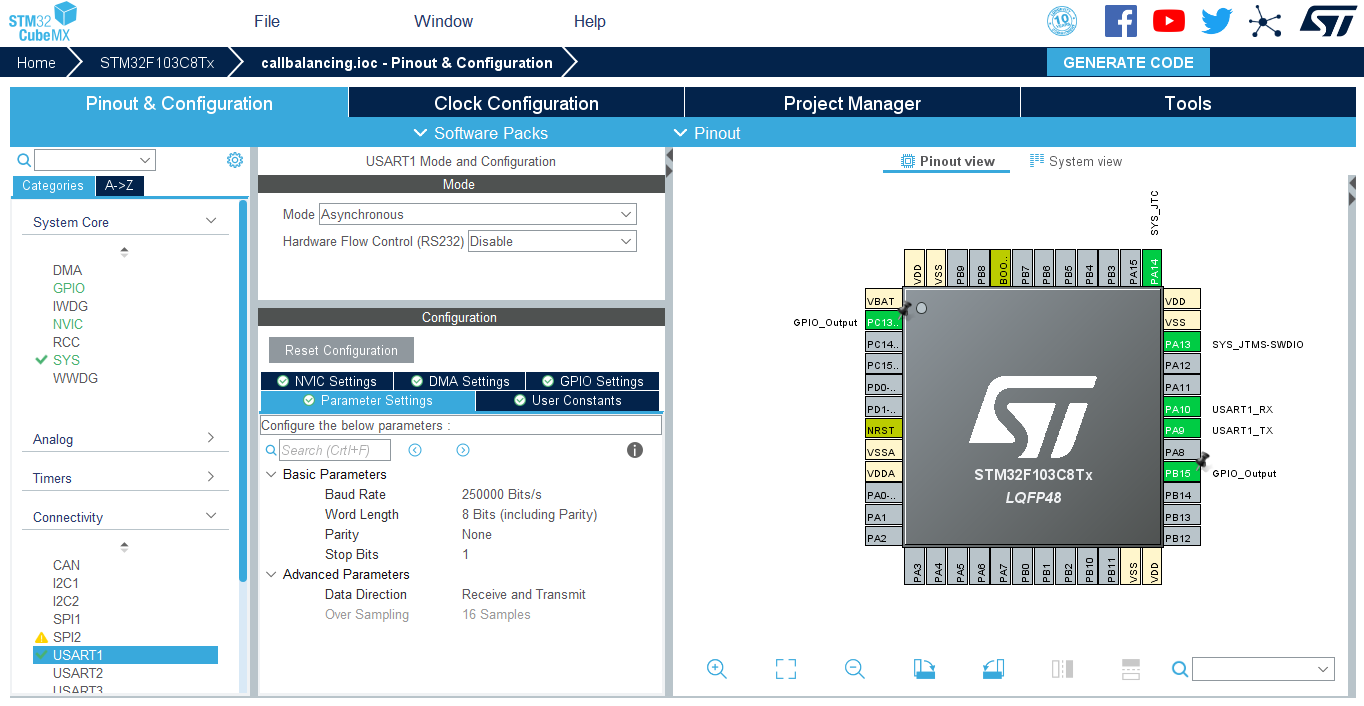
\includegraphics[scale=0.5]{Chapter4/cubemx.PNG}
    \caption{STM32CubeMX:Initialization code generator}
\end{figure}

The tool provides GUI interface tool select required microcontroller or microprocessor required by the user and rich easy-to-use graphical user interface allowing the configuration of pin-out with automatic conflict resolution, peripherals and middleware functional modes with dynamic validation of parameter constraints for Arm\textsuperscript{\textregistered} Cortex\textsuperscript{\textregistered}-M core, clock tree with dynamic validation of the configuration, and power sequence with estimated consumption results. After required configuration tool can generate initialization C code compliant with IAR™, Keil\textsuperscript{\textregistered} and STM32CubeIDE (GCC compilers) for Arm\textsuperscript{\textregistered}Cortex\textsuperscript{\textregistered}-M core and user can configure new peripherals if required in future and regenerate code without affecting user written code.

\subsection{Command Response Protocol for BQ76PL455A-Q1}
Command response protocol needs to be followed in order to communicate and control Battery monitoring \acrshort{ic}(s) BQ76PL455A-Q1 via \acrshort{uart} connection with a host microcontroller.Its is frame transaction based protocol with error detection using IBM16 Cyclic Redundancy check (\acrshort{crc}).The  protocols specifications is provided by Texas instruments in chip's datasheet \cite{ti:pl455}. The host microcontroller always need to initiate the communication by sending a command frame depending upon the request made a response frame might be received  from chip to host if command specifies request type as write with response.

\subsection{Transaction Frame Description}
The transaction frame format includes both Command Frames and Response Frames. There are five field types used within a transaction frame:

.\begin{itemize}
\item Frame Initialization
\item Device Address or Group ID
\item Register Address
\item Data
\item Cyclic Redundancy Check (\acrshort{crc})
\end{itemize}

\subsubsection{Frame Initialization}
The first byte of frame is called frame initialization byte. Since frame size is variable depending on data requested by the host, it is this byte which gives information about length of the frame and also 7\textsuperscript{th} bit of the byte provides information about whether the frame is command or response type. It also provide with other obvious information required in communication.Table 4.1 describes various fields in frame initialization byte.

\begin{table}[H]
  \centering
  
  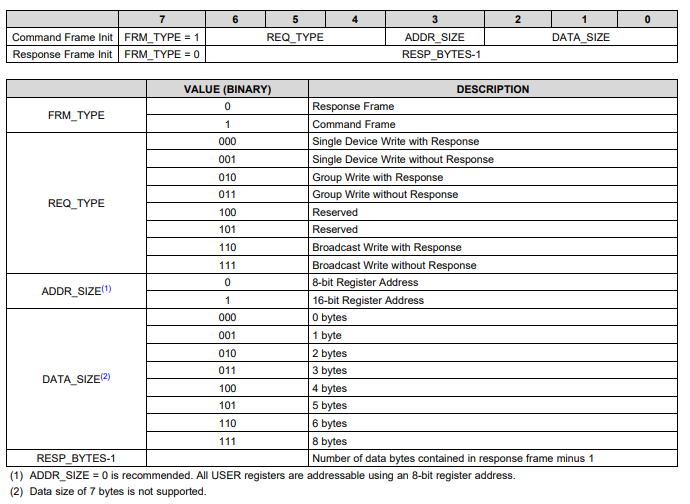
\includegraphics[]{Chapter4/Tables/frameinitbyte.PNG}
  \caption{Frame initialization byte table from \cite{ti:pl455}}
\end{table}

\subsubsection{Device Address or Group ID}
This field identifies the module in stack or the group of modules stacked. The module with matching address in their Device Address Register \cite{ti:pl455} will respond to the command The REQ\_TYPE field in the command frame will determine how to interpret this byte.

\subsubsection{Register Address}
The user can use one byte or two byte addressing as per needs but it is recommended to use one byte addressing \cite{ti:pl455}. The selection can be done by writing to ADDR\_SIZE field in frame initialisation byte. And the register map of the BQ76PL455 is provided in its datasheet\cite{ti:pl455}.

\subsubsection{Data field}
Data bytes in data field is interpreted as command if register addressed is Command Register (address 2) otherwise data is written/read to or from targeted register that depends on REQ\_TYPE mentioned in frame initialisation byte. If REQ\_TYPE is Write without Response, the data bytes contain the values to be written to the registers
or if REQ\_TYPE is Write with Response, the data bytes contain the values returned from the registers.

\subsubsection{Cyclic Redundancy Check (\acrshort{crc})}
The eight-data-bit \acrshort{uart} communication should be reliable as long as the difference between transmitter baud rate and receiver baud rate is less than 3.75\% \cite{uartrel}. And data sampled from a battery monitoring \acrshort{ic} is critical and any data error can trigger events which are not supposed to be triggered otherwise so \acrshort{crc} IBM 16 field is available in the frame in-order to ensure data correctness and integrity.

\subsection{Software Development for STM32 micro-controller}
Software development for STM32 was divided into two parts first Chip support library was written later using STM32CubeMX\textsuperscript{\textregistered} initialization code for microcontroller and using functions from CSL application code is written, The algorithm tested with Simulink\textsuperscript{\textregistered} is implemented in embedded C program.

\subsubection{BQ76PL455A-Q1 Chip support Library for STM32 family of micro-controllers}
A  Chip Support  Library for BQ76PL455A-Q1 is written for STM32 family of micro-controllers by referring software reference provided by Texas instruments \cite{ti:pl455example} and STM32 software manuals \cite{stm:halmanual}.The focus was to provide an API interface using functions so that engineers can make use of that to develop applications.And the library contains header and source files.

\paragraph{pl455.h} ~\linebreak
The header contains type definitions, and definitions for bit patterns needed by functions to build communication frames.And it also houses function prototypes defined in source file pl455.c . 

\lstinputlisting[language= C]{Chapter4/Code/pl455.h}
 
\paragraph{pl455.c} ~\linebreak
The source file contains definitions for functions declared in the header file pl455.h. Functions to build command frame, get cell voltages, reset communication with \acrshort{ic}, generate \acrshort{crc} for frame,power down and to wake up \acrshort{ic} from sleep is written.This functions can be called directly from main code hence not burdening application engineers.

\lstinputlisting[language= C]{Chapter4/Code/pl455.c}

\paragraph{main.c} ~\linebreak
The application code wakes up the \acrshort{ic}, checks fault flags, sample cell voltages read by battery monitoring \acrshort{ic}  and implements passive cell balancing algorithm. The number of cells (\acrshort{noc}) parameter can be changed based on number of cells in the pack and it supports up to 16 cells.

\lstinputlisting[language= C]{Chapter4/Code/main.c}

\vspace{2cm}

In this chapter the implementation of the balancing algorithm on a  microcontroller is discussed with the details of libraries developed for the battery monitoring \acrshort{ic} with STM32 family of microcontrollers. The balancing algorithm tested is implemented on STM32F103C8T6 using Keil software development tool. The next chapter gives a consolidated report of the results obtained during the course of the project.

